\documentclass{fefu_presentation}

\usepackage{nicefrac}
\usepackage{xcolor}
\usepackage{tikz}
\usepackage{mathtools}
\usepackage{multicol}
\usepackage{multirow}
\usepackage{bm}
\usepackage{qrcode}
\usepackage{subcaption}
\usepackage[backend=biber, bibstyle=gost-numeric, maxbibnames=99, sorting=none]{biblatex}
\usepackage{bibentry}
\usepackage{scrextend}
\usepackage{etoolbox}
\usepackage{forloop}
\usepackage{pgffor}
\addbibresource{../references.bib}


\usetikzlibrary{positioning,decorations,calc,arrows.meta,patterns.meta}
\graphicspath{{../images/}}

\definecolor{redish}{rgb}{0.8,0.2,0.2}
\definecolor{greenish}{rgb}{0,0.7,0.3}

\DeclareMathOperator*{\argmax}{arg\,max}

\newif\ifstartcompletesineup
\newif\ifendcompletesineup
\pgfkeys{
	/pgf/decoration/.cd,
	start up/.is if=startcompletesineup,
	start up=true,
	start up/.default=true,
	start down/.style={/pgf/decoration/start up=false},
	end up/.is if=endcompletesineup,
	end up=true,
	end up/.default=true,
	end down/.style={/pgf/decoration/end up=false}
}
\pgfdeclaredecoration{complete sines}{initial}
{
	\state{initial}[
	width=+0pt,
	next state=upsine,
	persistent precomputation={
		\ifstartcompletesineup
		\pgfkeys{/pgf/decoration automaton/next state=upsine}
		\ifendcompletesineup
		\pgfmathsetmacro\matchinglength{
			0.5*\pgfdecoratedinputsegmentlength / (ceil(0.5* \pgfdecoratedinputsegmentlength / \pgfdecorationsegmentlength) )
		}
		\else
		\pgfmathsetmacro\matchinglength{
			0.5 * \pgfdecoratedinputsegmentlength / (ceil(0.5 * \pgfdecoratedinputsegmentlength / \pgfdecorationsegmentlength ) - 0.499)
		}
		\fi
		\else
		\pgfkeys{/pgf/decoration automaton/next state=downsine}
		\ifendcompletesineup
		\pgfmathsetmacro\matchinglength{
			0.5* \pgfdecoratedinputsegmentlength / (ceil(0.5 * \pgfdecoratedinputsegmentlength / \pgfdecorationsegmentlength ) - 0.4999)
		}
		\else
		\pgfmathsetmacro\matchinglength{
			0.5 * \pgfdecoratedinputsegmentlength / (ceil(0.5 * \pgfdecoratedinputsegmentlength / \pgfdecorationsegmentlength ) )
		}
		\fi
		\fi
		\setlength{\pgfdecorationsegmentlength}{\matchinglength pt}
	}] {}
	\state{downsine}[width=\pgfdecorationsegmentlength,next state=upsine]{
		\pgfpathsine{\pgfpoint{0.5\pgfdecorationsegmentlength}{0.5\pgfdecorationsegmentamplitude}}
		\pgfpathcosine{\pgfpoint{0.5\pgfdecorationsegmentlength}{-0.5\pgfdecorationsegmentamplitude}}
	}
	\state{upsine}[width=\pgfdecorationsegmentlength,next state=downsine]{
		\pgfpathsine{\pgfpoint{0.5\pgfdecorationsegmentlength}{-0.5\pgfdecorationsegmentamplitude}}
		\pgfpathcosine{\pgfpoint{0.5\pgfdecorationsegmentlength}{0.5\pgfdecorationsegmentamplitude}}
	}
	\state{final}{}
}

\tikzset{
	between/.style args={#1 and #2}{
		at = ($(#1)!0.5!(#2)$)
	}
}

\tikzset{
	between base/.style args={#1 and #2}{
		between=#1.base and #2.base
	}
}

\defbibenvironment{betterlabel}
	{\list{}
		{%
			\setlength{\listparindent}{0cm}%
			\setlength{\leftmargin}{\bibhang}%
			\setlength{\itemindent}{\leftmargin}%
			\setlength{\itemsep}{\bibitemsep}%
			\setlength{\parsep}{\bibparsep}%
		}%
	}
	{\endlist}
	{\item[\textbullet]}

\newcommand{\pa}[1]{\left(#1\right)}
\newcommand{\dd}{\mathrm{d}}

\makeatletter
\setlength{\metropolis@progressinheadfoot@linewidth}{2pt}
\setlength{\metropolis@progressonsectionpage@linewidth}{2pt}
\makeatother

\setbeamersize{text margin left=3.5mm,text margin right=3.5mm}

\author{Тыщенко Андрей Геннадьевич}
\setfaculty{05.13.18 <<Математическое моделирование, численные методы и комплексы программ>>}
\setsupervisor{Петров Павел Сергеевич}{д.ф.-м.н.}
\title{Численное моделирование распространения широкополосных акустических сигналов и шумов в мелком море с использованием модовых параболических уравнений}

\fefuloadstyle{poi_phd_presentation}
\setdegree{к.ф.-м.н.}

%\newcommand{\forpoi}[1]{%
%	\AtEndDocument{#1}%
%}

\newcommand{\forpoi}[1]{#1}

\begin{document}
	\presentationtitlepage
	
	\nocite{*}
	
	\section{Введение}
	
	\begin{frame}[fragile]{Области применения моделирования звука}
		\begin{block}{}
			\vspace{-0.5cm}
			\begin{itemize}
				\item Оценка уровня антропогенных акустических шумов при выполнении сейсморазведочных работ на восточном шельфе о. Сахалин с целью защиты морских млекопитающих (в т. ч. краснокнижных серых китов)
				\item Определение зон акустической тени при выборе мест расположения источников навигационных сигналов
			\end{itemize}
		\end{block}
		\begin{block}{Трассировка лучей и гауссовых пучков}
			\begin{enumerate}
				\item BELLHOP3D, Porter M.
				\item TRACEO3D, Calazan R., Rodr\'iguez O.
			\end{enumerate}
		\end{block}
		\begin{block}{Модовое разложение}
			\begin{enumerate}
				\item KRAKEN3D, Porter M.
			\end{enumerate}
		\end{block}
		\begin{block}{Трёхмерное ПУ}
			\begin{enumerate}
				\item CAPRE3D, Duda T.
			\end{enumerate}
		\end{block}
%		\begin{figure}[h]
%			\includegraphics[width=0.7\textwidth]{sel.pdf}
%			\caption{Оценка уровня антропогенного шума}
%		\end{figure}
	\end{frame}
	
	\begin{frame}[fragile]{Звуковое поле}
		\begin{block}{Уравнение Гельмгольца}			
			\smallskip
			\begin{equation}
				\pa{\Delta + K^2\pa{x,y,z}}p\pa{x,y,z}=-\delta\pa{x}\delta\pa{y}\delta\pa{z-z_s}
			\end{equation}
			\begin{equation*}
				K\pa{x,y,z}=\frac{\omega}{c\pa{x,y,z}}\pa{1+i\eta\beta\pa{x,y,z}}
			\end{equation*}
			\vskip -1cm
			\begin{align*}
				p\bigr|_{z=0}&=0 &p\bigr|_{z=h^{-}}&=p\bigr|_{z=h^{+}}\\
				p\bigr|_{z=H}&=0 &\frac{1}{\rho}\frac{\partial p}{\partial\mathbf{n}}\biggr|_{z=h^{-}}&=\frac{1}{\rho}\frac{\partial p}{\partial\mathbf{n}}\biggr|_{z=h^{+}}\\
			\end{align*}
			\vskip -0.5cm
			\centering
			\begin{tabular}{lc}
				$\rho\pa{z}$ --- плотность среды & \multirow{5}{*}{
					\begin{tikzpicture}
						\coordinate (ORIGIN) at (-2, 0, 1.5);
						
						\coordinate (B100) at (-2, 0, 0);
						\coordinate (B200) at (2, 0, 0);
						\coordinate (B202) at (2, 0, 3);
						\coordinate (B102) at (-2, 0, 3);
						
						\coordinate (B120) at (-2, -2, 0);
						\coordinate (B220) at (2, -2, 0);
						\coordinate (B222) at (2, -2, 3);
						\coordinate (B122) at (-2, -2, 3);
						
						\draw[-] (B120) -- (B220) -- (B222) -- (B122) -- cycle;
						
						\draw[-] (B100) -- (B120);
						\draw[-] (B200) -- (B220);
						\draw[-] (B102) -- (B122);
					
						\fill[draw,preaction={fill=gray!40},pattern={Lines[angle=45,distance=5]}] (-2, -0.5, 3) -- (-0.5, -0.5, 3) -- (0.5, -1, 3) -- (2, -1, 3) -- (2, -1.5, 3) -- (0.5, -1.5, 3) -- (-0.5, -1, 3) -- (-2, -1, 3) -- cycle;
						
						\fill[draw,preaction={fill=gray!40},pattern={Lines[angle=60,distance=2.5]}] (2, -1, 3) -- (2, -1, 1.5) -- (2, -0.25, 0) -- (2, -0.75, 0) -- (2, -1.5, 1.5) -- (2, -1.5, 3) -- cycle;
						
						\fill[draw,fill=gray!40] (-2, -0.5, 3) -- (-2, -0.5, 0) -- (-0.5, -0.5, 0) -- (-0.5, -0.5, 3) -- cycle;
						\fill[draw,fill=gray!40] (-0.5, -0.5, 0) -- (2, -0.25, 0) -- (2, -1, 1.5) -- cycle;
						\fill[draw,fill=gray!40] (-0.5, -0.5, 3) -- (0.5, -1, 3) -- (0.5, -1, 1.5) -- (-0.5, -0.5, 0) -- cycle;
						\fill[draw,fill=gray!40] (0.5, -1, 3) -- (0.5, -1, 1.5) -- (2, -1, 1.5) --  (2, -1, 3) -- cycle;
						\fill[draw,fill=gray!40] (-0.5, -0.5, 0) --  (2, -1, 1.5) -- (0.5, -1, 1.5) -- cycle;
						
						\draw[-{Latex}, very thick] (ORIGIN) -- ++(1,0,0) node[below right=-1mm] {$x$};
						\draw[-{Latex}, very thick] (ORIGIN) -- ++(0,-1,0) node[above right] {$z$};
						\draw[-{Latex}, very thick] (ORIGIN) -- ++(0,0,1) node[above] {$y$};
						
						\draw[-] (B100) -- (B200) -- (B202) -- (B102) -- cycle;
						\draw[-] (B202) -- (B222);
						
						\fill[draw,preaction={fill=gray!60},pattern={Lines[angle=45,distance=3]}] (-2, -1, 3) -- (-0.5, -1, 3) -- (0.5, -1.5, 3) --  (2, -1.5, 3) -- (B222) -- (B122) -- cycle;
						
						\fill[draw,preaction={fill=gray!60},pattern={Lines[angle=60,distance=1.5]}] (2, -1.5, 3) -- (2, -1.5, 1.5) -- (2, -0.75, 0) -- (B220) -- (B222) -- cycle;
						
						\node at (-2.2, -0.5, 3) {$h_0$};
						\node at (-2.2, -1, 3) {$h_1$};
						\node at (-2.2, -2, 3) {$H$};
						
						\draw[fill=black] (ORIGIN) circle[radius=1mm];						
					\end{tikzpicture}
				}\\
				$c\pa{x,y,z}$ --- скорость звука & \\
				$\omega=2\pi f$ --- циклическая частота & \\
				$\beta$ --- коэффициент затухания & \\
				$\eta=\nicefrac{1}{40\pi\log_{10}e}$
			\end{tabular}
		\end{block}
	\end{frame}
	
	\begin{frame}[fragile]{Цель работы}
		\begin{block}{}
			Разработка эффективного метода моделирования распространения широкополосных акустических сигналов в трёхмерном волноводе мелкого моря и комплекса программ на основе этого метода, позволяющего решать широкий класс задач за разумное время
			\begin{itemize}
				\item Моделирование трёхмерного звукового поля с использованием модового разложения звука
				\item Трассировка лучей, соответствующих вертикальным модам
				\item Вычисление временного ряда импульса звукового сигнала в произвольных точках волновода с указанием опорного сигнала в одной из них или функции источника
				\item Расчёт интегральных характеристик (SEL)
			\end{itemize}
		\end{block}
	\end{frame}
	
	\section{Математические методы}
	
	\begin{frame}[fragile]{Модовое разложение поля}
		\begin{block}{Модовое разложение}
			\smallskip
			\begin{equation}
				p\pa{x,y,z}=\sum\limits_{j=1}^JA_j\pa{x,y}\varphi_j\pa{z,x,y}
			\end{equation}
		\end{block}
		\vskip -0.5cm
		\begin{block}{Спектральная задача}
			\smallskip
			\begin{equation}
				\begin{dcases}
					\frac{\dd^2\varphi\pa{z}}{\dd z^2}+K^2\pa{z}\varphi\pa{z}=k^2\varphi\pa{z}\,,\\
					\varphi\bigr|_{z=0}=0\,,\qquad \varphi\bigr|_{z=h^{-}}=\varphi\bigr|_{z=h^{+}}\,,\\
					\varphi\bigr|_{z=H}=0\,,\qquad \frac{1}{\rho}\frac{\dd \varphi}{\dd z}\bigr|_{z=h^{-}}=\frac{1}{\rho}\frac{\dd \varphi}{\dd z}\bigr|_{z=h^{+}}
				\end{dcases}
			\end{equation}
		\end{block}
		\begin{block}{Уравнение горизонтальной рефракции}
			\smallskip
			\begin{equation}
				\frac{\partial^2 A_j}{\partial x^2} + \frac{\partial^2 A_j}{\partial y^2}+k_j^2 (x,y)A_j=-\varphi_j(z_s)\delta(x)\delta(y)
			\end{equation}
		\end{block}
	\end{frame}
	
	\begin{frame}[fragile]{Псевдодифференциальное МПУ}
		\begin{block}{}
			\begin{equation}
				\pa{\frac{\partial}{\partial x}+i\sqrt{k_j^2\pa{x,y}+\frac{\partial^2}{\partial y^2}}}\underbrace{\pa{\frac{\partial}{\partial x}-i\sqrt{k_j^2\pa{x,y}+\frac{\partial^2}{\partial y^2}}}A_j\pa{x,y}}_{=0}=0\,,
			\end{equation}
		\end{block}
		\begin{block}{}
			\begin{equation}
				A_j\pa{x,y}=e^{k_{j,0}x}\mathcal{A}_j\pa{x,y}
			\end{equation}
			\begin{equation}
				\begin{dcases}
					\frac{\partial\mathcal{A}_j\pa{x,y}}{\partial x}=ik_{j,0}\pa{\sqrt{1+L_j}-1}\mathcal{A}_j\pa{x,y}\,,\\
					\mathcal{A}_j\pa{0,y}=\mathcal{A}_{j,0}\pa{y}
				\end{dcases}
			\end{equation}
			\begin{equation}
				k_{j,0}^2L_j=\frac{\partial^2}{\partial y^2}+k_j^2\pa{x,y}-k_{j,0}^2\nonumber
			\end{equation}	
		\end{block}
	\end{frame}
	
	\begin{frame}[fragile]{Аппроксимация оператора квадратного корня}
		\begin{block}{Аппроксимация Паде для функции $F\pa{\lambda}$}
			\smallskip
			\begin{equation}
				F\pa{\lambda}\approx\mathcal{R}\pa{F,l,m}\pa{\lambda}\equiv\frac{P^F_{l,m}\pa{\lambda}}{Q^F_{l,m}\pa{\lambda}}
			\end{equation}
			$P^F_{l,m}, Q^F_{l,m}$ -- полиномы порядка $l$ и $m$ соответственно
		\end{block}
		\bigskip
		\begin{block}{Широкоугольное МПУ с аппроксимацией Паде}
			\smallskip
			\begin{equation}
				\frac{\partial\mathcal{A}_j\pa{x,y}}{\partial x}=\frac{P_{l,m}\pa{L_j}}{Q_{l,m}\pa{L_j}}\mathcal{A}_j\pa{x,y}
			\end{equation}
		\end{block}
	\end{frame}
	
	\forpoi{
		\begin{frame}{Дискретизация по $x$}
			\begin{block}{Дискретизация Крэнка-Николсон}
				\smallskip
				\begin{equation}
					D_h^+\mathcal{A}_j^n=\frac{P_{l,m}\pa{L_j}}{Q_{l,m}\pa{L_j}}\mathcal{A}_j^{\nicefrac{n+1}{2}}
				\end{equation}
				\begin{align*}
					D_h^+\mathcal{A}_j=\frac{\mathcal{A}_j^{n+1}-\mathcal{A}_j^n}{h}\,,&&\mathcal{A}_j^{\nicefrac{n+1}{2}}=\frac{\mathcal{A}_j^{n+1}+\mathcal{A}_j^n}{2}\,,&&\mathcal{A}_j^n\sim\mathcal{A}_j\pa{x_n,y}\,,&&x=nh
				\end{align*}
			\end{block}
			\vskip -1cm
			\begin{block}{}
				\smallskip
				\begin{equation}
					\mathcal{A}_j^{n+1}=\frac{-hP_{l,m}\pa{L_j}-2Q_{l,m}\pa{L_j}}{~~~hP_{l,m}\pa{L_j}-2Q_{l,m}\pa{L_j}}\mathcal{A}_j^n=\frac{U_{l,m}\pa{L_j}}{W_{l,m}\pa{L_j}}\mathcal{A}_j^n
				\end{equation}
			\end{block}
			\begin{block}{Дискретизированное МПУ}
				\smallskip
				\begin{equation}\label{eq::DMPE}
					\begin{gathered}
						\mathcal{A}_j^{n+1}=\pa{a_{l,m}^0+\sum\limits_{i=1}^p\frac{a_{l,m}^i}{1+b_{l,m}^iL_j}}\mathcal{A}_j^n\\
						1\leqslant l\leqslant m
					\end{gathered}
				\end{equation}
			\end{block}
		\end{frame}
	}
	
	\begin{frame}[fragile]{Split-step Pad\'e}
		\begin{block}{Пропагатор по $x$}
			\smallskip
			\begin{equation}
				\mathcal{A}_j^{n+1}=e^{ik_{j,0}h\pa{\sqrt{1+L_j}-1}}\mathcal{A}_j^{n}
			\end{equation}
		\end{block}
		\begin{block}{Аппроксимация экспоненты квадратного корня}
			\smallskip
			\begin{equation}
				e^{ik_{j,0}h\pa{\sqrt{1+L_j}-1}}\approx\frac{\tilde{P}_{l,m}\pa{L_j}}{\tilde{Q}_{l,m}\pa{L_j}}=\tilde{a}_{l,m}^0+\sum\limits_{i=1}^m\frac{\tilde{a}_{l,m}^i}{1+\tilde{b}_{l,m}^iL_j}
			\end{equation}
		\end{block}
		\begin{block}{Дискретизированное МПУ}
			\smallskip
			\begin{equation}
				\begin{gathered}
					\mathcal{A}_j^{n+1}=\pa{\tilde{a}_{l,m}^0+\sum\limits_{i=1}^p\frac{\tilde{a}_{l,m}^i}{1+\tilde{b}_{l,m}^iL_j}}\mathcal{A}_j^n\\
					1\leqslant l\leqslant m
				\end{gathered}
			\end{equation}
		\end{block}
	\end{frame}
	
	\begin{frame}{Дискретизация оператора $L_j$}
		\begin{block}{Центральная разница на равномерной сетке}
			\smallskip
			\begin{equation}
				D_\delta^2\mathcal{A}_j^{n+1}=\frac{\mathcal{A}_j^{n+1,q+1}-2\mathcal{A}_j^{n+1,q}+\mathcal{A}_j^{n+1,q-1}}{\delta^2}\,,\quad q\in\mathbb{N}
			\end{equation}
			\begin{equation*}
				y_q=y_0+q\delta\,,\qquad\Delta y=\delta\,,\qquad\mathcal{A}_j^{n,q}\sim\mathcal{A}_j\pa{x_n,y_q}
			\end{equation*}
		\end{block}
		\begin{block}{Полностью дискретизированное МПУ}
			\smallskip
			\begin{equation}
				\begin{gathered}
					\mathcal{A}_j^{b+1,q}=\pa{a_{l,m}^0+\sum\limits_{i=1}^p\frac{a^i_{l,m}}{1+b^i_{l,m}L_j^\delta}}\mathcal{A}_j^{n,q}\\
					k_{j,0}^2L_j^\delta=D_\delta^2+k_j^2-k_{j,0}^2\\
					1\leqslant l\leqslant m
				\end{gathered}
			\end{equation}
		\end{block}
	\end{frame}
	
	\begin{frame}{Численная схема}
		\begin{block}{Форма решения}
			\begin{equation}
				\mathcal{A}_j^{n+1,q}=a_{l,m}^0\mathcal{A}_j^{n,q}+\sum\limits_{i=1}^pa_{l,m}^i\mathcal{B}_{j,i}^{n+1,q}=\pa{a_{l,m}^0+\sum\limits_{i=1}^p\frac{a_{l,m}^i}{1+b_{l,m}^iL_j^\delta}}\mathcal{A}_j^{n,q}
			\end{equation}
		\end{block}
		\begin{block}{Уравнение для $\mathcal{B}_{j,i}$}
			\smallskip
			\begin{equation}
				\pa{1+b_{l,m}^iL_j^\delta}\mathcal{B}_{j,i}^{n+1,q}=\mathcal{A}_j^{n,q}\,,\quad i=\overline{1,p}
			\end{equation}
		\end{block}
		\begin{block}{Трёхдиагональная матрица}
			\smallskip
			\begin{equation}
				\underset{\alpha_{j,i}}{\underbrace{\frac{b_{l,m}^i}{k_{j,0}^2\delta^2}}}\mathcal{B}_{j,i}^{n+1,q-1}+\underset{\beta_{j,i}}{\underbrace{\pa{1+\frac{b_{l,m}^i}{k_{j,0}^2}\pa{k_j^2-k_{j,0}^2-\frac{2}{\delta^2}}}}}\mathcal{B}_{j,i}^{n+1,q}+\underset{\gamma_{j,i}}{\underbrace{\frac{b_{l,m}^i}{k_{j,0}^2\delta^2}}}\mathcal{B}_{j,i}^{n+1,q+1}=\mathcal{A}_j^{n,q}
			\end{equation}
		\end{block}
	\end{frame}
	
	\begin{frame}[fragile]{Perfectly matching layers}
		\begin{figure}[t]
			\begin{tikzpicture}
				\coordinate(C11);
				\foreach \i in {2,...,7} {
					\pgfmathtruncatemacro\index{\i-1}
					\coordinate[right of=C1\index](C1\i);
				}
				\foreach \i in {2,...,4} {
					\pgfmathtruncatemacro\index{\i-1}
					\coordinate[below of=C\index1](C\i1);
					\foreach \j in {2,...,7} {
						\pgfmathtruncatemacro\index{\j-1}
						\coordinate[right of=C\i\index](C\i\j);
					}
				}
				\draw (C11) -- (C17);
				\draw (C11) -- (C41);
				\draw (C17) -- (C47);
				\draw[dashed] (C12) -- (C42);
				\draw[dashed] (C16) -- (C46);
				\draw[decorate, decoration={complete sines}] (C41) -- (C47);
				
				\node[above=0 of C12](Y0){$y_0$};
				\node[above=0 of C16](Y1){$y_1$};
				
				\node[above=0 of C11]{$-\varepsilon$};
				\node[above=0 of C17]{$+\varepsilon$};
				
				\node[between base=C24 and C34]{\Large $\Omega$};
				\node[between base=C21 and C32]{PML};
				\node[between base=C26 and C37]{PML};
				
				\coordinate[at=($(Y0.base)!0.4!(Y1.base)$)](YA1);
				\coordinate[at=($(Y0.base)!0.6!(Y1.base)$)](YA2);
				\draw[->] (YA1) -- (YA2) node[midway,yshift=2mm]{$y$};
				
				\coordinate[left=2mm of C11](X0);
				\coordinate[left=2mm of C41](X1);
				
				\coordinate[at=($(X0.base)!0.4!(X1.base)$)](XA1);
				\coordinate[at=($(X0.base)!0.6!(X1.base)$)](XA2);
				\draw[->] (XA1) -- (XA2) node[midway,xshift=-2mm]{$x$};
			\end{tikzpicture}
		\end{figure}
		\begin{block}{Оператор в PML области}
			\smallskip
			\begin{equation}
				k_{j,0}^2L_j^{PML}=\frac{1}{1+i\sigma\pa{y}}\frac{\partial}{\partial y}\frac{1}{1+i\sigma\pa{y}}\frac{\partial}{\partial y}+k_j^2+k_{j,0}^2
			\end{equation}
			\begin{equation}
				\sigma\pa{y}=\sigma_0\pa{\frac{\left|y-y_b\right|}{\varepsilon}}^3=\sigma_0\zeta^3\equiv\sigma\pa{\zeta}\,,\quad\zeta\in\left[0, 1\right]
			\end{equation}
		\end{block}
	\end{frame}
	
	\forpoi{
		\begin{frame}{Дискретизация оператора $L_j^{PML}$}
			\begin{block}{Уравнение для $\mathcal{B}_{j,i}$ в PML области}
				\smallskip
				\begin{equation}
					\begin{gathered}
						D^1_{\nicefrac{\delta}{2}}F^q=\frac{F^{q+\nicefrac{1}{2}}-F^{q-\nicefrac{1}{2}}}{\delta}\\
						\pa{1+b_{l,m}^i\prescript{q}{\delta}{L_j^{PML}}}\mathcal{B}_{j,i}^{n+1,q}=\mathcal{A}_j^{n,q}\,,\quad i=\overline{1,p}\\
						k_{j,0}^2\prescript{q}{\delta}{L_j^{PML}}=\frac{1}{1+i\beta\pa{y_q}}D_{\nicefrac{q}{2}}^1\pa{\frac{1}{1+i\beta\pa{y_q}}D_{\nicefrac{q}{2}}^1}+k_j^2-k_{j,0}^2
					\end{gathered}
				\end{equation}
			\end{block}
			\begin{block}{Численная схема в PML обасти}
				\begin{multline}
					\underset{\tilde{\alpha}_{j,i}^q}{\underbrace{\frac{b_{l,m}^i\mu_q\mu_{q-\nicefrac{1}{2}}}{k_0^2\delta^2}}}\mathcal{B}_{j,i}^{n+1,q-1}+\underset{\tilde{\beta}_{j,i}^q}{\underbrace{\pa{1+\frac{b_{l,m}^i}{k_{j,0}^2}\pa{k_j^2-k_{j,0}^2-\frac{\mu_q}{\delta^2}\pa{\mu_{q-\nicefrac{1}{2}}+\mu_{q+\nicefrac{1}{2}}}}}}}\mathcal{B}_{j,i}^{n+1,q}+\\\underset{\tilde{\gamma}_{j,i}^q}{\underbrace{\frac{b_{l,m}^i\mu_q\mu_{q+\nicefrac{1}{2}}}{k_0^2\delta^2}}}\mathcal{B}_{j,i}^{n+1,q+1}=\mathcal{A}_j^{n,q}
				\end{multline}
			\end{block}
		\end{frame}
	}
	
	\begin{frame}{Граничные условия прозрачности}
		\begin{block}{Уравнение для $\mathcal{B}_{j,i}$}
			\smallskip
			\begin{equation}
				k_{j,0}^2\mathcal{B}_{j,i}^{n+1,q}+b_{l,m}^iD_\delta^2\mathcal{B}_{j,i}^{n+1,q}+b_{l,m}^i\pa{k_j^2-k_{j,0}^2}\mathcal{B}_{j,i}^{n+1,q}=k_{j,0}^2\mathcal{A}_j^{n,q}
			\end{equation}
		\end{block}
		\begin{block}{$\mathcal{Z}$-преобразование}
			\smallskip
			\begin{equation}
				\mathcal{Z}\left\{\mathcal{A}_j^{n,q}\right\}=\hat{\mathcal{A}}_j^q\pa{\zeta}\coloneq\sum\limits_{n=0}^\infty\zeta^{-n}\mathcal{A}_j^{n,q}\,,\quad\zeta\in\mathbb{C}\,,\quad\left|\zeta\right|>R_{\hat{\mathcal{A}}_j^q}
			\end{equation}
		\end{block}
		\begin{block}{Тогда при условии $\mathcal{A}_j^{n,q}=\mathcal{B}_j^{n,q}=0,\forall n<0$}
			\smallskip
			\begin{equation}
				-\zeta b_{l,m}^iD_\delta^2\hat{\mathcal{B}}_{j,i}^q=\zeta k_{j,0}^2\hat{\mathcal{B}}_{j,i}^q+\zeta b_{l,m}^i\pa{k_j^2-k_{j,0}^2}\hat{\mathcal{B}}_{j,i}^q-k_{j,0}^2\hat{\mathcal{A}}_j^q
			\end{equation}
		\end{block}
		\begin{block}{Дополнительное уравнение}
			\smallskip
			\begin{equation}
				\zeta\hat{\mathcal{A}}_j^q=a_{l,m}^0\hat{\mathcal{A}}_j^q+\zeta\sum\limits_{i=1}^pa_{l,m}^i\hat{\mathcal{B}}_{j,i}^q
			\end{equation}
		\end{block}
	\end{frame}
	
	\begin{frame}{Граничные условия прозрачности}
		\begin{block}{Обозначим $\hat{\bm{\Psi}}_j^q=\pa{\hat{\mathcal{A}}_j^q,\hat{\mathcal{B}}_{j,1}^q,\dots,\hat{\mathcal{B}}_{j,p}^q}^T\in\mathbb{C}^{p+1}$}
			\smallskip
			\begin{equation}
				\mathbf{X}_jD_\delta^2\hat{\bm{\Psi}}_j^q=\mathbf{Y}_j\hat{\bm{\Psi}}_j^q
			\end{equation}
		\end{block}
		\vskip -1cm
		\begin{block}{}
			\begin{gather}
				\mathbf{X}_j\coloneq\begin{pmatrix}
					0 & -\zeta b_{l,m}^1&&\\
					\vdots& & \ddots&&\\
					0&&&-\zeta b_{l,m}^p\\
					\zeta&0&\dots&0
				\end{pmatrix}\\
				\mathbf{Y}_j\coloneq\begin{pmatrix}
					-k_{j,0}^2&\zeta k_{j,0}^2+\zeta b_{l,m}^1\pa{k_j^2-k_{j,0}^2}&&\\
					\vdots&&\ddots&\\
					-k_{j,0}^2&&&\zeta k_{j,0}^2+\zeta b_{l,m}^p\pa{k_j^2-k_{j,0}^2}\\
					a_{l,m}^0&\zeta a_{l,m}^1&\dots&\zeta a_{l,m}^p
				\end{pmatrix}
			\end{gather}
			\begin{equation*}
				\mathbf{X}_j,\mathbf{Y}_j\in\mathbb{C}^{\pa{p+1}\times\pa{p+1}}
			\end{equation*}
		\end{block}
	\end{frame}
	
	\begin{frame}{Граничные условия прозрачности}
		\begin{block}{Введём переменную $\hat{\bm{\xi}}_j^q\coloneq D_q^-\hat{\bm{\Psi}}_j^q$}
			\begin{gather}
				\underbrace{\begin{pmatrix}
						\mathbf{0} & \mathbf{X}_j\\
						\mathbf{I} & -\mathbf{I}\delta
				\end{pmatrix}}_{\mathbf{A}_j} D_\delta^+
				\begin{pmatrix}
					\hat{\bm{\Psi}}_j^q\\
					\hat{\bm{\xi}}_j^q
				\end{pmatrix}=
				\underbrace{\begin{pmatrix}
						\mathbf{Y}_j & \mathbf{0}\\
						\mathbf{0} & \mathbf{I}
				\end{pmatrix}}_{\mathbf{B}_j}
				\begin{pmatrix}
					\hat{\bm{\Psi}}_j^q\\
					\hat{\bm{\xi}}_j^q
				\end{pmatrix}\\
				D_q^-\hat{\bm{\Psi}}_j^q=\frac{\hat{\bm{\Psi}}_j^q-\hat{\bm{\Psi}}_j^{q-1}}{\delta}\qquad D_q^+\hat{\bm{\Psi}}=\frac{\hat{\bm{\Psi}}_j^{q+1}-\hat{\bm{\Psi}}_j^q}{\delta}\nonumber
			\end{gather}
		\end{block}
		\vskip -0.5cm
		\begin{block}{Решение системы}
			\begin{equation}
				\begin{pmatrix}
					\hat{\bm{\Psi}}_j^{q+1}\\
					\hat{\bm{\xi}}_j^{q+1}
				\end{pmatrix}=
				\pa{\mathbf{A}_j^{-1}\mathbf{B}_j+\mathbf{I}}
				\begin{pmatrix}
					\hat{\bm{\Psi}}_j^q\\
					\hat{\bm{\xi}}_j^q
				\end{pmatrix}\,.
			\end{equation}
		\end{block}
		\vskip -0.5cm
		\begin{block}{Жорданова форма}
			\begin{equation}
				\begin{gathered}
					\mathbf{J}_j=\begin{pmatrix}
						\mathbf{J}_j^1 & \mathbf{0}\\
						\mathbf{0} & \mathbf{J}_j^2
					\end{pmatrix}=
					\mathbf{P}_j\pa{\mathbf{A}_j^{-1}\mathbf{B}_j+\mathbf{I}}\mathbf{P}_j^{-1}\\
					\mathbf{J}_j^1,\mathbf{J}_j^2,\mathbf{P}_j\in\mathbb{C}^{\pa{p+1}\times\pa{p+1}}
				\end{gathered}
			\end{equation}
		\end{block}
	\end{frame}
	
	\begin{frame}{Граничные условия прозрачности}
		\begin{block}{\small Разложение решения по базису $\mathbf{P}_j^{-1}$}
			\begin{equation}
				\mathbf{P}_j^{-1}\begin{pmatrix}
					\hat{\bm{\Psi}}_j^{q+1}\\
					\hat{\bm{\xi}}_j^{q+1}
				\end{pmatrix}=
				\mathbf{P}_j^{-1}\pa{\mathbf{A}_j^{-1}\mathbf{B}_j+\mathbf{I}}\begin{pmatrix}
					\hat{\bm{\Psi}}_j^q\\
					\hat{\bm{\xi}}_j^q
				\end{pmatrix}=
				\begin{pmatrix}
					\mathbf{J}_j^1 & \mathbf{0}\\
					\mathbf{0} & \mathbf{J}_j^2
				\end{pmatrix}
				\begin{pmatrix}
					\mathbf{P}_j^1\hat{\bm{\Psi}}_j^q+\mathbf{P}_j^2\hat{\bm{\xi}}_j^q\\
					\mathbf{P}_j^3\hat{\bm{\Psi}}_j^q+\mathbf{P}_j^4\hat{\bm{\xi}}_j^q
				\end{pmatrix}
			\end{equation}
		\end{block}
		\vskip -0.5cm
		\begin{block}{\small Потребуем равенству нулю решений возрастающих при $q\to\infty$}
			\vskip -0.5cm
			\begin{gather}
				\mathbf{P}_j^3\hat{\bm{\Psi}}_j^Q+\mathbf{P}_j^4\hat{\bm{\xi}}_j^Q=0\\
				D_\delta^-\hat{\bm{\Psi}}_j^Q=-\pa{\mathbf{P}_j^4}^{-1}\mathbf{P}_j^3\hat{\bm{\Psi}}_j^Q=\hat{\mathbf{D}}_j\hat{\bm{\Psi}}_j^Q
			\end{gather}
		\end{block}
		\vskip -0.5cm
		\begin{block}{\small Применив обратное преобразование получим}
			\begin{equation}
				\begin{gathered}
					\bm{\Psi}_j^{n+1,Q}-\bm{\Psi}_j^{n+1,Q-1}=\sum\limits_{l=1}^{n}\mathbf{D}_j^{n+1-l}\bm{\Psi}_j^{l,Q}\\
					\bm{\Psi}_j^{n,q}=\pa{\mathcal{A}_j^{n,q},\mathcal{B}_{j,1}^{n,q},\dots,\mathcal{B}_{j,1}^{n,q}}^T\in\mathbb{C}^{p+1}\\
					\mathbf{D}_j^n=\mathcal{Z}^{-1}\left\{\hat{\mathbf{D}}_j\pa{\zeta}\right\}=\frac{\tau^n}{2\pi}\int\limits_0^{2\pi}\hat{\mathbf{D}}_j\pa{\tau e^{i\phi}}e^{in\phi}\dd\phi\,,\quad n\in\mathbb{Z}_0\,,\quad\tau > 0
				\end{gathered}
			\end{equation}
		\end{block}
	\end{frame}
	
	\forpoi{	
		\begin{frame}{Лучевая теория распространения звука}
			\begin{block}{}
				\begin{equation}
					\mathcal{A}_j\pa{x,y}=M_j\pa{x,y}e^{ik_{j,0}S_j\pa{x,y}}+o\pa{\nicefrac{1}{k_{j,0}}}
				\end{equation}
			\end{block}
			\begin{block}{Уравнение Гамильтона-Якоби}
				\smallskip
				\begin{equation}
					\pa{\frac{\partial S_j\pa{x,y}}{\partial x}}^2+\pa{\frac{\partial S_j\pa{x,y}}{\partial y}}^2=n_j\pa{x,y}
				\end{equation}
				\begin{equation*}
					n_j\pa{x,y}\equiv \nicefrac{k_j\pa{x,y}}{k_{j,0}}
				\end{equation*}
			\end{block}
			\begin{block}{Уравнение переноса}
				\begin{multline}
					2\pa{\frac{\partial S_j\pa{x,y}}{\partial x}\frac{\partial M_j\pa{x,y}}{\partial x}+\frac{\partial S_j\pa{x,y}}{\partial y}\frac{\partial M_j\pa{x,y}}{\partial y}}+\\\pa{\frac{\partial^2S_j\pa{x,y}}{\partial x^2}+\frac{\partial^2S_j\pa{x,y}}{\partial y^2}}M_j\pa{x,y}=0
				\end{multline}
			\end{block}
		\end{frame}
	}
	
	\forpoi{
		\begin{frame}{Лучевая теория распространения звука}
			\begin{block}{Гамильтонова система}
				\smallskip
				\begin{equation}
					\begin{aligned}
						\begin{dcases}
							\frac{dx_j\pa{l}}{dl}=\frac{\xi_j\pa{l}}{n_j\pa{x_j,y_j}}\\
							x_j\pa{0}=0
						\end{dcases}&\qquad
						\begin{dcases}
							\frac{d\xi_j\pa{l}}{dl}=\frac{\partial n_j\pa{x_j,y_j}}{\partial x_j}\\
							\xi_j\pa{0}=\cos\alpha
						\end{dcases}\\
						&&\\
						\begin{dcases}
							\frac{dy_j\pa{l}}{dl}=\frac{\eta_j\pa{l}}{n_j\pa{x_j,y_j}}\\
							y_j\pa{0}=y_s
						\end{dcases}&\qquad
						\begin{dcases}
							\frac{d\eta_j\pa{l}}{dl}=\frac{\partial n_j\pa{x_j,y_j}}{\partial y_j}\\
							\eta_j\pa{0}=\sin\alpha
						\end{dcases}
					\end{aligned}
				\end{equation}
			\end{block}
		\end{frame}
	}
	
	\begin{frame}{Лучевые начальные условия}
		\begin{block}{Начальное условие}
			\smallskip
			\begin{gather}
				\mathcal{A}_j\pa{x_0,y}=M_j\pa{x_0,y}e^{ik_{j,0}S_j\pa{x_0,y}}\,,\qquad y_0\leqslant y\leqslant y_1\\
				S_j\pa{l}=\int\limits_0^ln_j\pa{l}dl\\
				M_j\pa{l}=\frac{M_{j,0}}{n_j\pa{l}}\sqrt{\frac{\cos\alpha}{\nicefrac{\partial y\pa{l,\alpha}}{\partial\alpha}}}\\
				M_{j,0}=\frac{e^\frac{i\pi}{4}}{\sqrt{8\pi k_{j,0}}}\nonumber
			\end{gather}
		\end{block}
		\vspace{-0.5cm}
		\begin{block}{Простые начальные условия}
			\smallskip
			\begin{equation}
				l=\sqrt{x_0^2+y^2}\,,\quad S\pa{l}=l\,,\quad M_j\pa{l}=\frac{M_{j,0}}{\sqrt{l}}
			\end{equation}
		\end{block}
	\end{frame}
	
	\begin{frame}{Временной ряд импульсного акустического сигнала}
		\begin{block}{Спектр импульса}
			\smallskip
			\begin{equation}
				\hat{I}_r\pa{\xi}=\overline{\hat{P}\pa{x_r,y_r,z_r,\xi}\cdot e^{-i\tau\omega\pa{\xi}}}
			\end{equation}
			\begin{equation}
				\hat{P}\pa{x,y,z,\xi}=p\pa{x,y,z,f\pa{\xi}}\cdot\overline{\hat{g}}\pa{\xi}
			\end{equation}
		\end{block}
		\begin{block}{Sound Exposure Level}
			\begin{equation}
				SEL\pa{x,y,z,f_1,f_2}=10\log_{10}\pa{\int\limits_{f_1}^{f_2}\left|\hat{P}\pa{x,y,z,\xi\pa{f}}\right|^2df}
			\end{equation}
		\end{block}
		\vspace{-0.5cm}
		\begin{figure}[h]
			\centering
			\includegraphics[width=0.7\textwidth]{impulse.pdf}
			\caption{Сигнал во временной области}
		\end{figure}
	\end{frame}
	
	\begin{frame}{Колебательное ускорение}
		\begin{block}{}
	       \begin{equation}
				\overline{a}=\left\{a_x,a_y,a_z\right\}=\left\{-\frac{1}{\rho}\frac{\partial p}{\partial x}, -\frac{1}{\rho}\frac{\partial p}{\partial y},-\frac{1}{\rho}\frac{\partial p}{\partial z}\right\}=-\frac{1}{\rho}\nabla p
	        \end{equation}
		\end{block}
	\begin{block}{}
		\begin{gather}
			\frac{\partial p}{\partial x}=\sum\limits_{j=1}^J\frac{\partial}{\partial x}\pa{e^{ik_{j,0}x}\mathcal{A}_j\varphi_j}=\sum\limits_{j=1}^Je^{ik_{j,0}x}\pa{ik_{j,0}\mathcal{A}_j\varphi_j+\frac{\partial}{\partial x}\pa{\mathcal{A}_j\varphi_j}}\\
			\frac{\partial p}{\partial y}=\sum\limits_{j=1}^Je^{ik_{j,0}x}\frac{\partial}{\partial y}\pa{\mathcal{A}_j\varphi_j}\\
			\frac{\partial p}{\partial z}=\sum\limits_{j=1}^Je^{ik_{j,0}x}\frac{\partial}{\partial z}\pa{\mathcal{A}_j\varphi_j}
	        \end{gather}
	   \end{block}
	\end{frame}
	
	\forpoi{
		\begin{frame}{Численное дифференцирование}
			\begin{block}{}
				\begin{equation}
					\mathfrak{A}_j=\mathcal{A}_j\varphi_j\nonumber
				\end{equation}
			\end{block}
			\vskip -1cm
			\begin{block}{}
				\begin{align}
					\frac{\partial\mathfrak{A}_j}{\partial x}\approx\mathcal{D}_{j,x}^{n,m,l}=\Delta x^{-1}&\begin{dcases}
						-3\mathfrak{A}_{j}^{1,m,l}+4\mathfrak{A}_{j}^{2,m,l}-\mathfrak{A}_{j}^{3,m,l},& n=1,\\
						\mathfrak{A}_{j}^{3,m,l} - \mathfrak{A}_{j}^{1,m,l},& n=2,\\
						\mathfrak{A}_{j}^{n - 2,m,l}-4\mathfrak{A}_{j}^{n - 1,m,l}+3\mathfrak{A}_{j}^{n,m,l},& else
					\end{dcases}\\
					\frac{\partial\mathfrak{A}_j}{\partial y}\approx\mathcal{D}_{j,y}^{n,m,l}=\Delta y^{-1}&\begin{dcases}
						-3\mathfrak{A}_{j}^{n,1,l}+4\mathfrak{A}_{j}^{n,2,l}-\mathfrak{A}_{j}^{n,3,l},& m=1,\\
						\mathfrak{A}_{j}^{n,m-2,l}-4\mathfrak{A}_{j}^{n,m-1,l}+3\mathfrak{A}_{j}^{n,m,l},& m=ny,\\
						\mathfrak{A}_{j}^{n,m+1,l}-\mathfrak{A}_{j}^{n,m-1,l},& else
					\end{dcases}\\
					\frac{\partial\mathfrak{A}_j}{\partial z}\approx\mathcal{D}_{j,z}^{n,m,l}=\Delta z^{-1}&\begin{dcases}
						-3\mathfrak{A}_{j}^{n,m,1}+4\mathfrak{A}_{j}^{n,m,2}-\mathfrak{A}_{j}^{n,m,3},& l=1,\\
						\mathfrak{A}_{j}^{n,m,l-2}-4\mathfrak{A}_{j}^{n,m,l-1}+3\mathfrak{A}_{j}^{n,m,l},& l=nz,\\
						\mathfrak{A}_{j}^{n,m,l+1} - \mathcal{B}_{j}^{n,m,l-1},& else
					\end{dcases}
				\end{align}
			\end{block}
		\end{frame}
	}
	
	\begin{frame}{Выводы}
		\begin{block}{}
			Было рассмотрено вычисление решения уравнения Гельмгольца с использованием широкоугольных модовых параболических уравнений в адиабатическом приближении и предложена численная схема их решения, основанная на применении аппроксимации Паде к пропагатору. Введены согласованные поглощающие слои и граничные условия прозрачности. Рассмотрено вычисление верменного ряда импульсного акустического сигнала, SEL и колебательных ускорений.
		\end{block}
	\end{frame}
	
	\section{Программная реализация}
	
	\begin{frame}{Комплекс программ}
		\begin{block}{}
			\begin{itemize}
				\item Язык C++20
				\item Репозиторий: {\footnotesize \url{https://github.com/GoldFeniks/AMPLE}}
				\item 162 коммита, \textcolor{greenish}{++}18028, \textcolor{redish}{\textminus\textminus}8505
				\item Зависимости
				\begin{itemize}
					\item Boost C++
					\item ALGLIB
					\item fftw3
					\item nlohmann::json
					\item Eigen
				\end{itemize}
				\item Модули
				\begin{itemize}
					\item CAMBALA\qquad {\footnotesize \url{https://github.com/Nauchnik/Acoustics-at-home/}}
					\item DORK\qquad {\footnotesize \url{https://github.com/GoldFeniks/DORK}}
					\item delaunay\qquad {\footnotesize \url{https://github.com/GoldFeniks/delaunay}}
					\item zip\qquad {\footnotesize \url{https://github.com/GoldFeniks/zip}}
				\end{itemize}
			\end{itemize}
		\end{block}
		\begin{tikzpicture}[remember picture,overlay]
			\node[xshift=-1.75cm,yshift=-2.75cm] at (current page.north east){\qrcode[height=2.5cm]{https://github.com/GoldFeniks/AMPLE}};
		\end{tikzpicture}
	\end{frame}
	
	\begin{frame}{Возможности разработанного комплекса программ}
		\vskip -0.75cm
		\begin{block}{}
			\begin{itemize}
				\item Вычисление трёхмерного поля звукового давления на основе решения широкоугольных модовых параболических уравнений
				\item Вычисление вертикальных мод на основе заданных параметров среды (гидрология, батиметрия, параметры слоёв) или использование предрасчитанных значений
				\item Проведение трассировки горизонтальных лучей, соответствующих вертикальным модам
				\item Вычисление временного ряда импульса звукового сигнала в произвольных точках среды и SEL
				\item Вычисление поля колебательных ускорений
				\item Реализация лучевых начальных условий и PML
				\item Высокая скорость работы за счёт использования параллельных вычислений
				\item Конфигурация вычислений с использованием текстового файла в формате JSON
			\end{itemize}
		\end{block}
	\end{frame}
	
	\begin{frame}{Входные и выходные данные}
		\begin{block}{Входные данные}
			\begin{itemize}
				\item config.json
				\item Дополнительные текстовые или бинарные файлы
				\vspace{-0.25cm}
				\begin{multicols}{2}
					\begin{itemize}
						\item Модовые функции и собственные значения
						\item Частоты
						\item Батиметрия
					\end{itemize}
					\columnbreak
					\begin{itemize}
						\item Гидрология
						\item Координаты приёмников
						\item Функция и спектр источника
					\end{itemize}
				\end{multicols}
			\end{itemize}
		\end{block}
		\begin{block}{Выходные данные}
			\begin{itemize}
				\item meta.json
				\item config.json
				\item Файлы вывода
				\item Папки вывода нескольких фалов {\small\ttfamilylatin <job\_type>/meta.json}
			\end{itemize}
		\end{block}
	\end{frame}
	
	\begin{frame}[fragile]{Волновод Пекериса}
		\begin{figure}[h]
			\centering
			\vskip -0.25cm
			\begin{subfigure}[t]{0.35\textwidth}
				\centering
				\includegraphics[width=\textwidth]{pekeris.pdf}
				\caption{Аналитическое решение}
			\end{subfigure}
			\begin{subfigure}[t]{0.35\textwidth}
				\centering
				\includegraphics[width=\textwidth]{pekeris_wampe.pdf}
				\caption{Решение ШМПУ}
			\end{subfigure}\\
			\begin{subfigure}[t]{0.35\textwidth}
				\centering
				\includegraphics[width=\textwidth]{pekeris_n5.pdf}
				\caption{SSP, $p=5$}
			\end{subfigure}
			\begin{subfigure}[t]{0.35\textwidth}
				\centering
				\includegraphics[width=\textwidth]{pekeris_n17.pdf}
				\caption{SSP, $p=17$}
			\end{subfigure}
			\vskip -0.25cm
			\caption{Акустическое поле в волноводе Пекериса}
		\end{figure}
	\end{frame}
	
	\begin{frame}[fragile]{Принцип работы PML граничных условий}
		\begin{figure}[h]
			\centering
			\includegraphics[width=0.7\textwidth]{pekeris_pml_n13.pdf}
			\caption{Акустическое поле в волноводе Пекериса на глубине $z=30\ \text{м.}$, слои PML отмечены красной пунктирной линией, ширина слоёв составляет $1$ километр, порядок аппроксимации Паде $p=13$}
		\end{figure}
	\end{frame}
	
	\begin{frame}[fragile]{Подводный каньон}
		\vspace{-0.25cm}
		\begin{figure}[h]
			\centering
			\includegraphics[width=0.3\textwidth]{canyon_transparent.png}
			\caption{Схематичное изображение волновода}
		\end{figure}
		\vspace{-0.75cm}
		\begin{figure}[h]
			\centering
			\includegraphics[width=0.75\textwidth]{canyon_n11.pdf}
			\caption{Акустическое поле в волноводе с подводным каньоном}
		\end{figure}
	\end{frame}
	
	\begin{frame}[fragile]{Подводный каньон. Сравнительный анализ}
		\begin{figure}[h]
			\centering
			\includegraphics[width=0.9\textwidth]{canyon_compare.pdf}
			\caption{Сравнение результатов вычисления акустического поля в мелком море с подводным каньоном при $y=0\ \text{км.}$ на глубине $z=10\ \text{м}$.}
		\end{figure}
	\end{frame}
	
	\begin{frame}[fragile]{Клиновидный волновод}
		\vspace{-0.25cm}
		\begin{figure}[h]
			\centering
			\includegraphics[width=0.3\textwidth]{wedge_transparent.png}
			\caption{Схематичное изображение волновода}
		\end{figure}
		\vspace{-0.75cm}
		\begin{figure}[h]
			\centering
			\begin{subfigure}[t]{0.35\textwidth}
				\centering
				\includegraphics[width=\textwidth]{wedge_wampe.pdf}
				\caption{Решение ШМПУ}
			\end{subfigure}
			\begin{subfigure}[t]{0.35\textwidth}
				\centering
				\includegraphics[width=\textwidth]{wedge_n13.pdf}
				\caption{SSP}
			\end{subfigure}
			\caption{Акустическое поле в клиновидном волноводе}
		\end{figure}
	\end{frame}
	
	\begin{frame}[fragile]{Клиновидный волновод. Сравнительный анализ}
		\begin{figure}[h]
			\centering
			\vspace{-0.25cm}
			\begin{tikzpicture}
				\node (IMG) at (0,0) {\includegraphics[width=0.6\textwidth]{wedge_comp_1.pdf}};
				\node[left=.5cm of IMG]{\textbf{(a)} $x=\ 1\ \text{км.}$};
			\end{tikzpicture}
			\begin{tikzpicture}
				\node (IMG) at (0,0) {\includegraphics[width=0.6\textwidth]{wedge_comp_9.pdf}};
				\node[left=.5cm of IMG]{\textbf{(b)} $x=\ 9\ \text{км.}$};
			\end{tikzpicture}
			\begin{tikzpicture}
				\node (IMG) at (0,0) {\includegraphics[width=0.6\textwidth]{wedge_comp_17.pdf}};
				\node[left=.45cm of IMG]{\textbf{(c)} $x=25\ \text{км.}$};
			\end{tikzpicture}
			\caption{Сравнение результатов вычисления акустического поля вдоль $y$}
		\end{figure}
	\end{frame}
	
	\begin{frame}[fragile]{Клиновидный волновод. Сравнительный анализ}
		\begin{figure}[h]
			\centering
			\begin{subfigure}[t]{0.55\textwidth}
				\centering
				\includegraphics[width=\textwidth]{wedge_comp.pdf}
			\end{subfigure}
			\hfill
			\begin{subfigure}[t]{0.55\textwidth}
				\centering
				\includegraphics[width=\textwidth]{wedge_comp_close.pdf}
			\end{subfigure}
			\caption{Сравнение результатов вычисления акустического поля вдоль $x$}
		\end{figure}
	\end{frame}
	
	\forpoi{%
		\begin{frame}{Волновод с реальной батиметрией}
			\vspace{-0.25cm}
			\begin{multicols}{2}
				\begin{figure}[h]
					\centering
					\includegraphics[width=0.4\textwidth]{sakhalin_transparent.png}
					\caption{Рельеф дна}
				\end{figure}
				\columnbreak
				\begin{figure}[h]
					\centering
					\includegraphics[width=0.33\textwidth]{sound_profile.pdf}
					\caption{Скорость звука}
				\end{figure}
			\end{multicols}
			\begin{block}{Функция скорости звука}
				\smallskip
				\begin{equation}
					c\pa{z}=1491-\frac{29}{1+\exp\pa{6-\frac{12z}{21}}}
				\end{equation}
			\end{block}
		\end{frame}
	}
	
	\forpoi{%
		\begin{frame}{\normalsize Волновод с реальной батиметрией. Акустическое поле источника}
			\begin{figure}[h]
				\centering
				\begin{subfigure}{.6\textwidth}
					\centering
					\includegraphics[width=\textwidth]{sakhalin_wampe_z4.pdf}
					\caption{Решение ШМПУ}
				\end{subfigure}
				\begin{subfigure}{.6\textwidth}
					\centering
					\includegraphics[width=\textwidth]{sakhalin_n11_z4.pdf}
					\caption{Решение SSP}
				\end{subfigure}
			\end{figure}
		\end{frame}
	}
	
	\begin{frame}{Выводы}
		Выполнена программная реализация описанных математических методов. Большое внимание было уделено простоте конфигурации расчётов и скорости вычислений. Исходный код программы расмещён в открытом доступе. Проведена валидачия разработанной программы на модельных примерах.
	\end{frame}
	
	\section{Моделирование акустических полей в задачах оценки уровней антропогенных шумов в океане}
	
	\begin{frame}{Моделирование шума одиночного судна}
		\begin{block}{Выисляемые величины}
			\vskip -0.5cm
			\begin{gather}
				E_{p,ddec}\pa{f_c,d} = 2\int_{f_1}^{f_2} |\hat{P}\pa{f,d}|^2 df\\
				\bar{p^2}_{ddec}\pa{f} = \nicefrac{E_{p,ddec}\pa{f_c,d_{CPA}}}{T}
			\end{gather}
			\centering
			\small
			\begin{tabular}{ll}
				$f_c$ -- центральная частота полосы $\left[f_1,f_2\right]$ & $d$ -- растояние до источника\\
				$d_{CPA}$ -- расстояние до ближ. точки прохода & $T=1 \text{с}$ -- размер временного окна
			\end{tabular}
		\end{block}
		\vskip -0.5cm
		\begin{figure}[h]
			\centering
			\includegraphics[width=0.95\textwidth]{d1/bath.pdf}
			\vskip -0.25cm
			\caption{Карта глубин акватории вблизи станции мониторинга и траектория прохода судна}
		\end{figure}
	\end{frame}
	
	\begin{frame}{Первые результаты моделирования}
		\begin{figure}[h]
			\centering
			\begin{subfigure}[t]{0.7\textwidth}
				\centering
				\includegraphics[width=\textwidth]{d1/target.pdf}
				\caption{Данные}
			\end{subfigure}
			\vskip -0.5cm
			\begin{subfigure}[t]{0.7\textwidth}
				\centering
				\includegraphics[width=\textwidth]{d1/ample_non_optimized.pdf}
				\caption{Моделирование}
			\end{subfigure}
			\vskip -0.5cm
			\caption{Уровни шума (в дБ) для прохождения судна}
		\end{figure}
	\end{frame}
	
	\begin{frame}{Исследование источника ошибки}
		\begin{figure}[h]
			\centering
			\includegraphics[width=\textwidth]{d1/cross_non_optimized_400.pdf}
			\caption{Вертикальный срез акустического поля для частоты $f=400\text{ Гц}$ (в Дб. отн. 1 м. от источника)}
		\end{figure}
	\end{frame}
	
	\begin{frame}{Оптимизация параметров среды}
		\begin{block}{Байесовская оптимизация}
			\begin{enumerate}
				\item Для целевой функции $f: \Theta\mapsto\mathbb{R}$ получить априорное распределение $p\pa{f|\theta\in\Theta}$
				\item Вычислить $n\in\mathbb{N}$ значений целевой функции $y_i=f\pa{\theta_i}$ в случайно выбранных точках $\left\{\theta_i\right\}_{i=1}^n$
				\item Получить апостериорное распределение $p\pa{f|\theta_1,\dots,\theta_n,y_1,\dots,y_n}$
				\item Для каждого $j=\overline{1,m}\,,m\in\mathbb{N}$ выполнить
				\begin{enumerate}
					\item Получить следующую лучшую точку $\theta_{n+j}$ путём максимизации некоторой функции оценки $q: \Theta\mapsto\mathbb{R}$
					\item Вычислить значение целевой функции в новой найденной точке $y_{n+j}=f\pa{\theta_{n+j}}$.
					\item Обновить апостериорное распределение $p\pa{f|\theta_1,\dots,\theta_{n+j},y_1,\dots,y_{n+j}}$.
				\end{enumerate}
				\item Выдать максимальное значение $y_{max}=\max\limits_{i=\overline{1,n+m}}y_i$ и соответствующую ему точку $\theta_{max}=\argmax\limits_{\theta_i,i=\overline{1,n+m}}y_i$
			\end{enumerate}
		\end{block}
	\end{frame}
	
	\begin{frame}{Оптимизируемые параметры}
		\small
		\begin{table}[h]
			\centering
			\begin{subtable}[h]{\textwidth}
				\centering
				\begin{tabular}{|c|c|c|c|c|c|}
					\hline
					\multirow{3}{*}{} & \multicolumn{5}{c|}{Слой осадков}\\
					\cline{2-6}
					& \multirow{2}{*}{\begin{tabular}{@{}c@{}}Толщина \\ $\Delta z, \text{м}$\end{tabular}} &
					\multicolumn{2}{c|}{\begin{tabular}{@{}c@{}}Скорость звука \\ $\text{м}/\text{с}$\end{tabular}} &
					\multirow{2}{*}{\begin{tabular}{@{}c@{}}Плотность \\ $\text{г}/\text{см}^3$\end{tabular}} &
					\multirow{2}{*}{\begin{tabular}{@{}c@{}}Коэфф. погл. \\$\text{дБ}/\lambda$\end{tabular}}\\
					\cline{3-4}
					& & $c$ & $\Delta c$ & & \\
					\hline
					исходные & $50$ & $1541$ & $50$ & $1.8$ & $0.61$\\
					\hline
					оптим. & $61.4$ & $1519.2$ & $50$ & $2$ & $2.01$\\
					\hline
					диапазон & $\left[20,200\right]$ & $\left[1500,1600\right]$ & $\left[0,100\right]$ & $\left[1,2\right]$ & $\left[0.1,2.5\right]$\\
					\hline
				\end{tabular}
			\end{subtable}
			\vskip -0.5cm
			\begin{subtable}[h]{\textwidth}
				\centering
				\vspace{1cm}
				\begin{tabular}{|c|c|c|c|c|}
					\hline
					\multirow{2}{*}{} & \multicolumn{3}{c|}{Слой основания} & \multirow{2}{*}{\begin{tabular}{@{}c@{}} Профиль\\ скорости звука\\ в воде \end{tabular}}\\
					\cline{2-4}
					& \begin{tabular}{@{}c@{}}Скорость звука \\ $\text{м}/\text{с}$\end{tabular} &
					\begin{tabular}{@{}c@{}}Плотность \\ $\text{г}/\text{см}^3$\end{tabular} &
					\begin{tabular}{@{}c@{}}Коэфф. погл. \\ $\text{дБ}/\lambda$\end{tabular}&\\
					\hline
					исходные. & $2160$ & $2$ & $0.25$ & 0\\
					\hline
					оптим. & $1931.5$ & $2$ & $0.25$& -1\\
					\hline
					диапазон & $\left[1800,3000\right]$ & & & $\left[-1,1\right]$\\
					\hline
				\end{tabular}
			\end{subtable}
			\caption{Оптимизируемые параметры}
		\end{table}
	\end{frame}
	
	\begin{frame}{Результаты оптимизации}
		\begin{figure}[h]
			\centering
			\includegraphics[width=0.6\textwidth]{d1/compare.pdf}
			\caption{График зависимости распределения шума от частоты в точке ближайшего прохода судна}
		\end{figure}
	\end{frame}
	
	\begin{frame}{Результаты моделирования}
		\vskip -0.25cm
		\begin{figure}[h]
			\centering
			\begin{subfigure}[h]{0.7\textwidth}
				\centering
				\includegraphics[width=\textwidth]{d1/cross_non_optimized_400.pdf}
				\caption{Исходные параметры}
			\end{subfigure}
			\vskip -0.25cm
			\begin{subfigure}[h]{0.7\textwidth}
				\centering
				\includegraphics[width=\textwidth]{d1/cross_optimized_400.pdf}
				\caption{Оптимизированные параметры}
			\end{subfigure}
			\vskip -0.25cm
			\caption{Вертикальный срез акустического поля для частоты $f=400\text{ Гц}$ (в Дб. отн. 1 м. от источника)}
		\end{figure} 
	\end{frame}
	
	\begin{frame}{Результаты моделирования}
		\vskip -0.25cm
		\begin{figure}[h]
			\centering
			\begin{subfigure}[h]{0.7\textwidth}
				\centering
				\includegraphics[width=\textwidth]{d1/ample_non_optimized.pdf}
				\caption{Исходные параметры}
			\end{subfigure}
			\vskip -0.5cm
			\begin{subfigure}[h]{0.7\textwidth}
				\centering
				\includegraphics[width=\textwidth]{d1/ample_epddec.pdf}
				\caption{Оптимизированные параметры}
			\end{subfigure}
			\vskip -0.25cm
			\caption{Уровни шума (в дБ) для прохождения судна}
		\end{figure} 
	\end{frame}
	
	\begin{frame}{Результаты моделирования}
		\vskip -0.25cm
		\begin{figure}[h]
			\centering
			\begin{subfigure}[t]{0.7\textwidth}
				\centering
				\includegraphics[width=\textwidth]{d1/flat_epddec.pdf}
				\caption{2D}
				\label{fig::noise_ddec_opt_2d}
			\end{subfigure}
			\vskip -0.5cm
			\begin{subfigure}[t]{0.7\textwidth}
				\centering
				\includegraphics[width=\textwidth]{d1/ample_epddec.pdf}
				\caption{3D}
			\end{subfigure}
			\vskip -0.25cm
			\caption{Уровни шума (в дБ) для прохождения судна}
		\end{figure}
	\end{frame}
	
	\begin{frame}{Точность моделирования}
		\vskip -0.25cm
		\begin{figure}[h]
			\centering
			\begin{subfigure}[t]{0.7\textwidth}
				\centering
				\includegraphics[width=\textwidth]{d1/non_optimzied_20.pdf}
				\caption{Исходные параметры}
			\end{subfigure}
			\vskip -0.25cm
			\begin{subfigure}[t]{0.7\textwidth}
				\centering
				\includegraphics[width=\textwidth]{d1/optimzied_20.pdf}
				\caption{Оптимизированные параметры}
			\end{subfigure}
			\vskip -0.25cm
			\caption{График точности моделирования уровней шумов}
		\end{figure}
	\end{frame}
	
	\forpoi{
		\begin{frame}{Задача мониторинга сейсморазведочных работ}
			\begin{figure}[H]
				\centering
				\includegraphics[width=0.8\textwidth]{seismo/pic_map.eps}
				\caption{Карта глубин в области проведения сейсморазведочных работ и график зависимости скорости звука от глубины}
			\end{figure}
		\end{frame}
	
		\begin{frame}{Задача мониторинга сейсморазведочных работ}
			\begin{figure}[h]
				\centering
				\includegraphics[width=0.8\textwidth]{seismo/pic_signal2.eps}
				\caption{Изменение акустического давления в приёмниках P1 и P2 и их спектры}
			\end{figure}
		\end{frame}
		
		\begin{frame}{Задача мониторинга сейсморазведочных работ}
			\begin{figure}[h]
				\centering
				\includegraphics[width=0.8\textwidth]{seismo/pic_waveguide.eps}
				\caption{Модель волновода и значения акустических параметров среды}
			\end{figure}
		\end{frame}
		
		\begin{frame}{Упрощённая модель батиметрии}
			\begin{figure}[h]
				\centering
				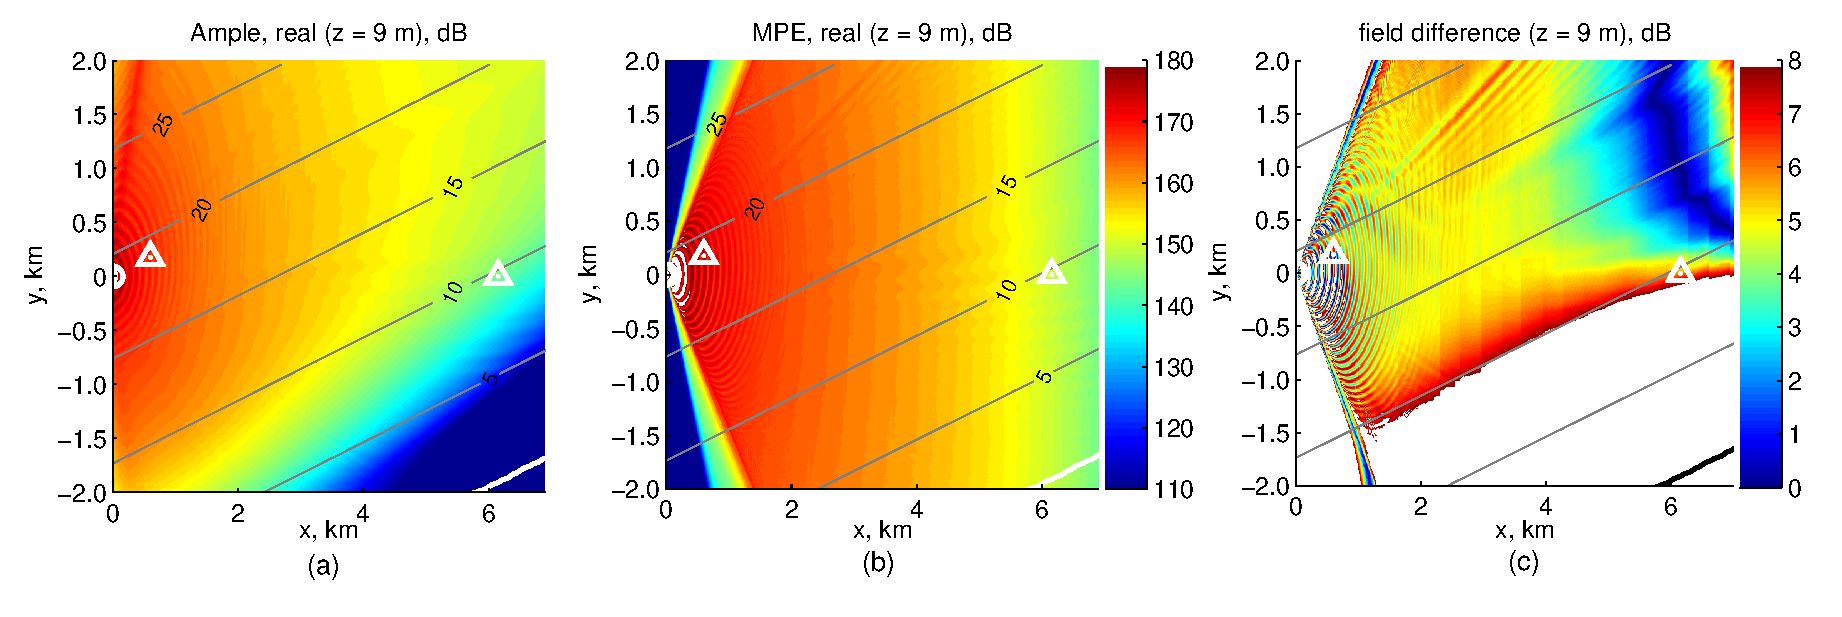
\includegraphics[width=0.95\textwidth]{seismo/pic_lineField.eps}
				\caption{Пространственное распределение уровня звуковой экспозиции при глубине 9 м в волноводе с упрощённой батиметрией}
			\end{figure}
		\end{frame}
		
		\begin{frame}{Реальная батиметрия}
			\begin{figure}[h]
				\centering
				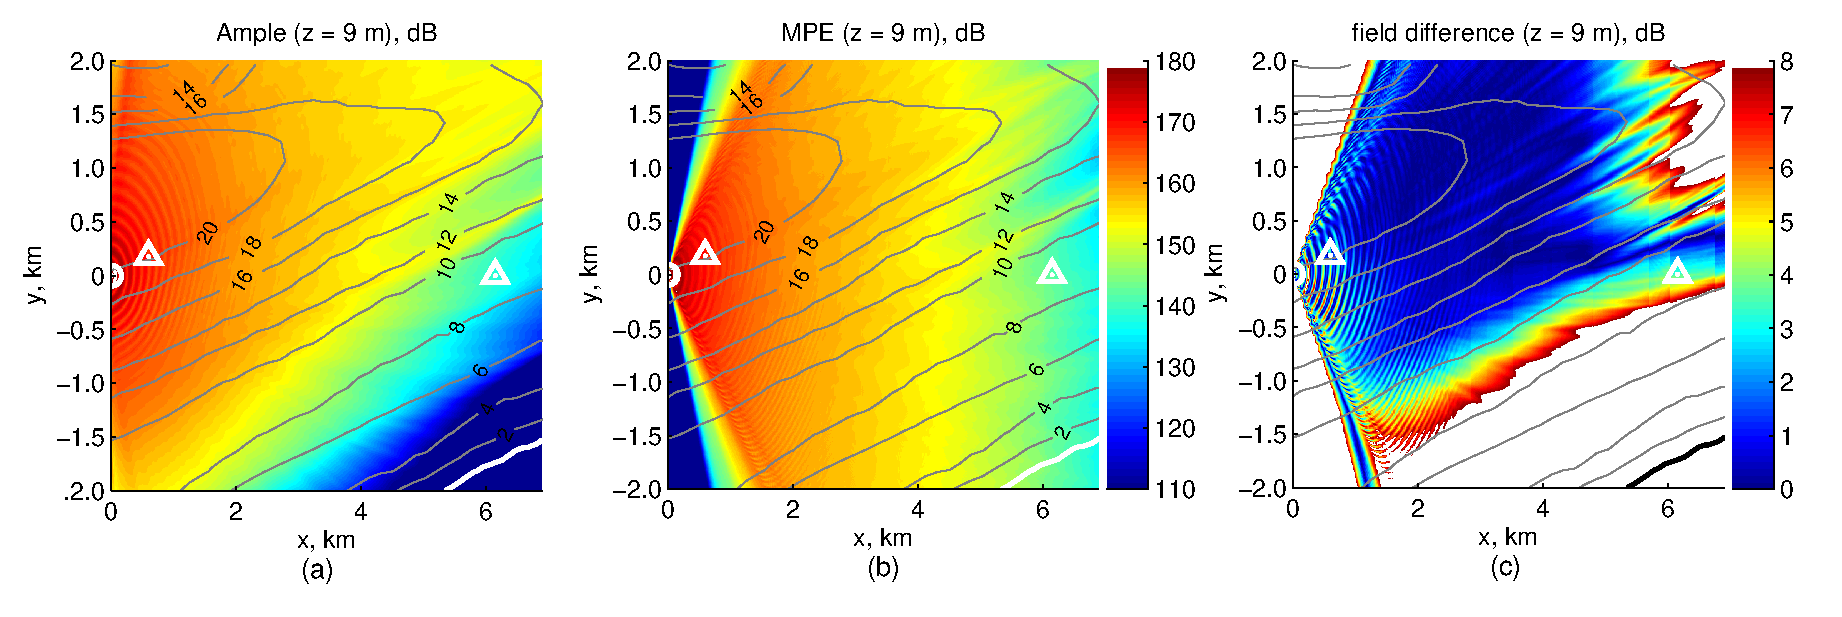
\includegraphics[width=0.95\textwidth]{seismo/pic_realField.eps}
				\caption{Пространственное распределение уровня звуковой экспозиции при глубине 9 м в волноводе с реальной батиметрией}
			\end{figure}
		\end{frame}
		
		\begin{frame}{Результаты моделирования}
			\begin{figure}[h]
				\centering
				\includegraphics[width=0.8\textwidth]{seismo/pic_test_sel.eps}
				\caption{График зависимости уровня звуковой экспозиции от расстояния $x$ на прямой $y=0$ и глубине 9 м}
			\end{figure}
		\end{frame}
		
		\begin{frame}{Результаты моделирования}
			\begin{figure}[h]
				\centering
				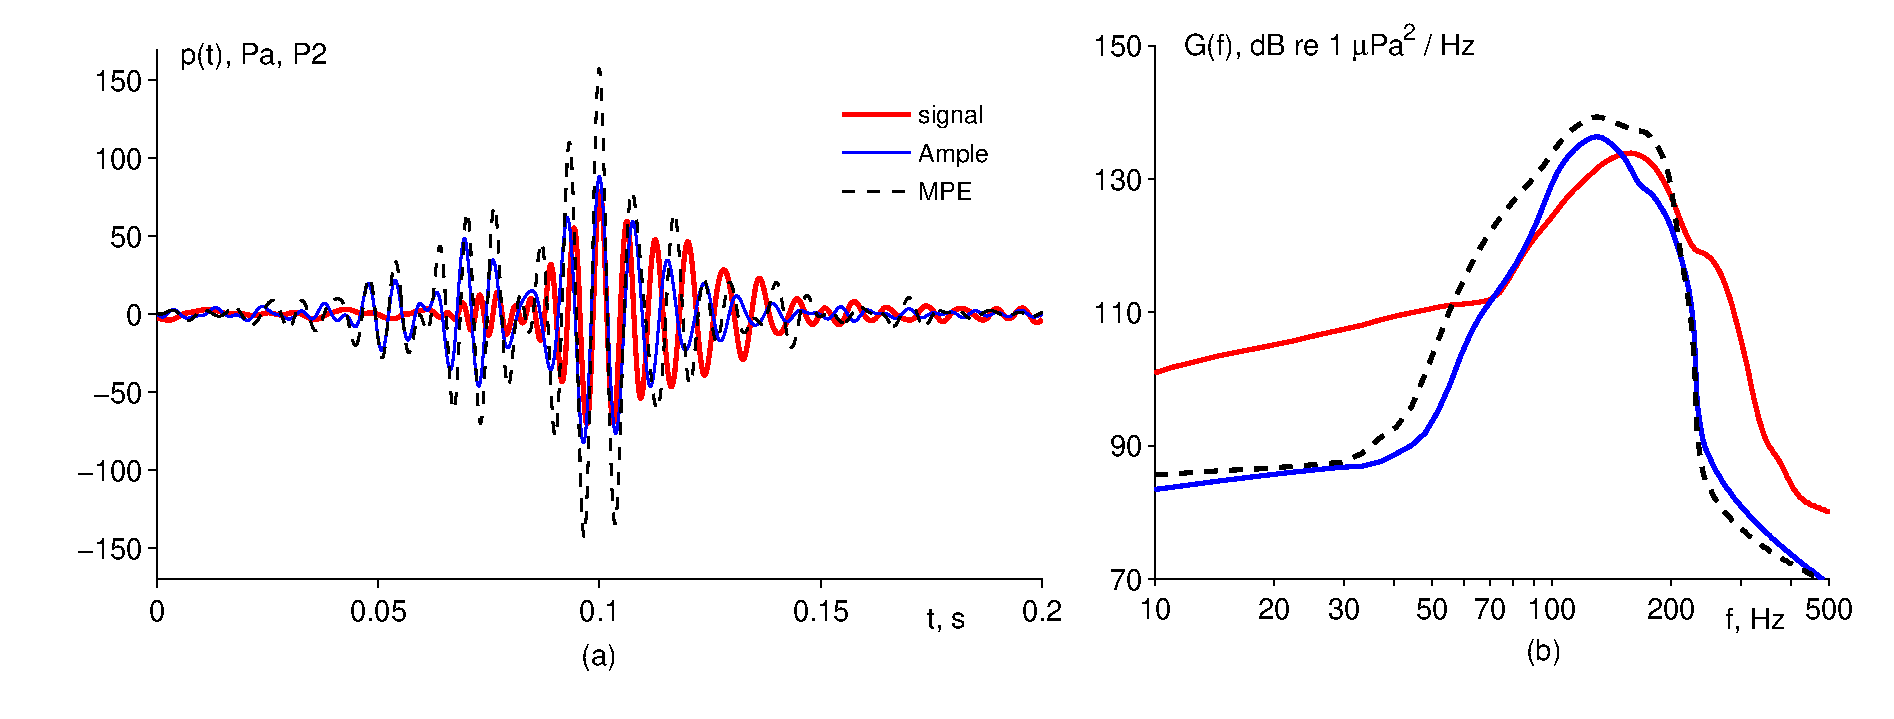
\includegraphics[width=0.9\textwidth]{seismo/pic_signal3.eps}
				\caption{Сравнение импульсных сигналов (\textbf{a}) и их спектров (\textbf{b})}
			\end{figure}
		\end{frame}
	}
	
	\begin{frame}{Выводы}
		\begin{block}{}
			Проведено моделирование акустических полей в задачах оценки уровней антропогенных шумов. Предложен способ оптимизации парамектров среды и показана его эффективность. Исследована важность использования широкоугольного уравнения.
		\end{block}
	\end{frame}
	
	\begin{frame}{Положения, выносимы на зашиту}
		\vskip -1cm
		\begin{block}{}
			\footnotesize
			\begin{enumerate}
				\item Разработана и апробирована методика численного решения псевдодифференциальных модовых параболических уравнений с искусственным ограничением расчётной области путём постановки граничных условий прозрачности или добавления к ней согласованных поглощающих слоёв
				\item Разработан комплекс программ на языке программирования C++, который может быть использован для моделирования распространения тональных и импульсных сигналов, а также вычисления скалярных и векторных акустических полей антропогенных шумов в океане с возможностью учёта батиметрических и гидрологических данных и структуры слоёв дна, и ориентированный на максимальную производительность
				\item Моделирование антропогенных шумов, связанных с сейсморазведочными работами и судоходством, проведённое с использованием разработанного комплекса прикладных программ, позволило добиться согласия уровней акустической экспозиции (SEL) с данными прямых измерений с точностью до 1 дБ. и согласия значений распределения энергии в децидекадных частотных полосах на различных расстояниях от источника шума с точностью до 5 дБ. для диапазона частот, в котором сосредоточена большая часть энергии сигнала
			\end{enumerate}
		\end{block}
	\end{frame}
	
	\begin{frame}{Научные труды. Статьи}
		\AtNextBibliography{\changefontsizes{8pt}}
		\printbibliography[heading=none,env=betterlabel,keyword={myarticles}]
	\end{frame}
	
	\begin{frame}{Научные труды. Материалы конференций}
		\AtNextBibliography{\changefontsizes{8pt}}
		\printbibliography[heading=none,env=betterlabel,keyword={myproceedings}]
	\end{frame}
	
	\begin{frame}
		\thispagestyle{empty}
		\addtocounter{framenumber}{-1}
		\centerline{\Huge Спасибо за внимание}
	\end{frame}
	
\end{document}
